\documentclass[letterpaper,12pt]{article}
\usepackage{ifthen}
\usepackage{times}
\usepackage{amsmath}
\usepackage{amssymb}
\usepackage{helvet}
\usepackage{courier}
\usepackage{fancyheadings}
\usepackage{hyperref}
\usepackage{comment}
\pagestyle{fancy}
\usepackage{pmc}
\usepackage{graphicx}
\setlength\textwidth{6.5in}
\setlength\textheight{8.5in}

%%%%%%%%%%%%%%%%%%%%%%%%%%%%%%%%%%%%%%%%%%%%%%%%%%%%%%%%%%%%%%%%%%%%%%%%%%%%%%%%%%
% Special for e-unibus doc commands

\newcommand{\ForLater}{
\begin{center}
{\bf NOT FOR CURRENT VERSION}
\end{center}
}
\newcommand{\TBC}{\framebox{\textbf{TO BE COMPLETED}}}
\newcommand{\DISCUSS}{\Ovalbox {\bf \textcolor{red}{FOR DISCUSSION}}}
\newcommand{\Input}{\framebox{\textsf{in}}}
\newcommand{\Output}{\framebox{\textsf{out}}}
\newcommand{\debug}[1]{\textbf{debug start} #1 \textbf{debug finish}}
\newcommand{\inx}[1]{\emph{#1}}
\newtheorem{notation}{Notation}
\newtheorem{definition}{Definition}
\newtheorem{problem_statement}{Problem Statement}
\newtheorem{invariant}{Invariant}
\newtheorem{assumption}{Assumption}
\newtheorem{resource_string}{Resource String}
\newtheorem{testcase}{Test Case}
\newtheorem{note}{Note}
\newtheorem{specification}{Specification}
\newtheorem{caution}{Caution}
\newtheorem{prereq}{Pre-requisite}
\newtheorem{action}{Action}
\newtheorem{query}{Query}
\newcommand{\beq}{\begin{equation}} %% new, no conflict
\newcommand{\eeq}{\end{equation}} %% new, no conflict
\newcommand{\be}{\begin{enumerate}}
\newcommand{\ee}{\end{enumerate}}
\newcommand{\bi}{\begin{itemize}}
\newcommand{\ei}{\end{itemize}}
\newcommand{\bv}{\begin{verbatim}}
\newcommand{\ev}{\end{verbatim}}
\newcommand{\bd}{\begin{description}}
\newcommand{\ed}{\end{description}}
\newcommand{\bpre}{\begin{prereq}}
\newcommand{\epre}{\end{prereq}}
\newcommand{\bact}{\begin{action}}
\newcommand{\eact}{\end{action}}
\newcommand{\bs}{\begin{specification}}
\newcommand{\es}{\end{specification}}
\newcommand{\btc}{\begin{testcase}}
\newcommand{\etc}{\end{testcase}}
\newcommand{\bc}{\begin{caution}}
\newcommand{\ec}{\end{caution}}
\newcommand{\la}{\leftarrow}
\newcommand{\IpArgs}{\subsection{Input Arguments}}
\newcommand{\PreReqs}{\subsection{Pre-requisities}}
\newcommand{\Actions}{\subsection{Actions}}
\newcommand{\Coverage}{{\bf To test coverage.}}

%%%%%%%%%%%%%%%%%%%%%%%%%%%%%%%%%%%%%%%%%%%%%%%%%%%%%%%%%%%%%%%%%%%%%%%%%%%


\newtheorem{theorem}{Theorem}[section]
\newtheorem{lemma}[theorem]{Lemma}
\newtheorem{proposition}[theorem]{Proposition}
\newtheorem{corollary}[theorem]{Corollary}

\newenvironment{proof}[1][Proof]{\begin{trivlist}
\item[\hskip \labelsep {\bfseries #1}]}{\end{trivlist}}
\newenvironment{intuition}[1][Intuition]{\begin{trivlist}
\item[\hskip \labelsep {\bfseries #1}]}{\end{trivlist}}
%% \newenvironment{definition}[1][Definition]{\begin{trivlist}
%% \item[\hskip \labelsep {\bfseries #1}]}{\end{trivlist}}
\newenvironment{example}[1][Example]{\begin{trivlist}
\item[\hskip \labelsep {\bfseries #1}]}{\end{trivlist}}
\newenvironment{remark}[1][Remark]{\begin{trivlist}
\item[\hskip \labelsep {\bfseries #1}]}{\end{trivlist}}

\newcommand{\qed}{\nobreak \ifvmode \relax \else
      \ifdim\lastskip<1.5em \hskip-\lastskip
      \hskip1.5em plus0em minus0.5em \fi \nobreak
      \vrule height0.75em width0.5em depth0.25em\fi}

%%%%%%%%%%%%%%%%%%%%%%%%%%%%%%%%%%%%%%%%%%%%%%%%%%%%%%%%%%%%%%%%%
% \newcommand{\Alogon}{\mbox{\fontfamily{ptm}\selectfont {\large \selectfont A} \hspace{-1.2ex} {\large \selectfont L} \hspace{-2.3ex} \raisebox{0.45ex}{ {\footnotesize \selectfont O} } \hspace{-1.80ex} {\large \selectfont G} \hspace{-1.80ex} \raisebox{-0.33ex}{ {\large \selectfont O} } \hspace{-1.8ex} {\large \selectfont N}}}



\newcommand{\beq}{\begin{equation}} %% new, no conflict
\newcommand{\eeq}{\end{equation}} %% new, no conflict
\newcommand{\bdm}{\begin{displaymath}} %% new, no conflict
\newcommand{\edm}{\end{displaymath}} %% new, no conflict
% \newcommand{\reals}{{\rm I\! R}} %% new, no conflict
\newcommand{\reals}{\cal{R}} %% new, no conflict
% \newcommand{\mymean}[1]{\mu({#1})}
\newcommand{\bb}[1]{\mathbf{#1}}
\newboolean{longform}
\setboolean{longform}{false}
\newboolean{blogpost}
\setboolean{blogpost}{true}
%% Another option is \usepackage{comment}
%% \includecomment(answer} or excludecomment{answer} % then
%% \begin{answer} ... \end{answer}


%% From https://math.berkeley.edu/~gbergman/misc/hacks/langl_rangl.html
\newcommand{\langl}{\begin{picture}(4.5,7)
\put(1.1,2.5){\rotatebox{60}{\line(1,0){5.5}}}
\put(1.1,2.5){\rotatebox{300}{\line(1,0){5.5}}}
\end{picture}}

\newcommand{\rangl}{\begin{picture}(4.5,7)
\put(.9,2.5){\rotatebox{120}{\line(1,0){5.5}}}
\put(.9,2.5){\rotatebox{240}{\line(1,0){5.5}}}
\end{picture}}

\newcommand{\mymean}[1]{\ensuremath{\langl{#1}\rangl}} %% new, no conflict

\begin{document}
\title{Analysis of Binary Outcome A/B Tests - New Metrics and a Bayesian Approach}
\author{ Ramesh Subramonian, Ranjeet Tate, Michael Shire, Abhi Singh}
\maketitle
\thispagestyle{fancy}
\lhead{}
\chead{}
\rhead{}
\lfoot{}
% \cfoot{{\small NerdWallet Engineering }}
% \rfoot{{\small \thepage}}

In a {\em binary} experiment, each trial has only two possible
outcomes, a {\em success} (1) or a {\em failure} (0).  A population
being experimented on has a ``true'' probability of success \(p\)
which is to be inferred from the results of the test.

In an A/B test there are two populations or branches, each of which is
exposed to a different treatment. The populations have true success
probabilities \(p_A\) and \(p_B\). After a period of time
pre-determined by (``power'' calculations or otherwise), the
experiment will yield a count of the trials and successes in each
branch, \((n_A, m_A)\) and \((n_B, m_B)\). From this data we infer a
likelihood on {\em 2-dimensional probability space} \(\{(p_A,p_B)\}\).

Typically, analysis produces a probabilistic statement of the type
``11.1\% gain at 90\% confidence''.  The {\em goal of our analysis is
  to provide the client with a definite recommendation about choosing
  \(A\) or \(B\)}\footnote{Paraphrasing from Klugman {\em et al}
  ``Loss Models'', 2nd Ed. Wiley (2004), pg. 419: ``...the process
  must end with a winner. While qualifications, caveats etc. are often
  necessary, a commitment is required.''.} based on identified
business needs, using the data and justified by statistics.

We all agree that the criterion for acceptance should be decided on
before the experiment is started. Most decision makers do not want to
be faced with having to come up with a two-dimensional decision
criterion of minimum gain and minimum confidence (similar to the
statement above) before the experiment, but they or their business
analysts can easily produce a single-valued acceptance criterion, say
``10\% gain''. So let's give them what they need, a yes or no answer
based on a single number.

For testing the simple hypothesis that ``A is better than B'' it is
enough to consider the {\em difference} between success probabilities
---i.e. \(p_A-p_B>0\). However, there are situations where it is not
enough that A be simply better than B: due to capital or recurring
costs the client may want A to be better than B by some non-zero
amount. The Optimizely book on A/B testing includes an example of a
test comparing a page with a static ad to one with a
video\footnote{``Fail Fast and Learn'', pg. 79, {\em A/B Testing}, Dan
  Siroker and Pete Koomen, Wiley (2013)}. The variant with the video
was better in terms of both click-through and conversion rates, but
the costs of producing the video and displaying it were deemed ``too
high'' to launch the video version at scale. So in addition to being
statistically significant, the difference has to be {\em important}
enough to recommend proceeding.

But now the analyst faces a choice of {\em metric} by which to compare
\(p_A\) and \(p_B\). E.g., in order to trigger a recommendation, do we
want the {\em difference} between success probabilities to exceed
\(0.1\) ---i.e. \(p_A-p_B>0.1\)--- or do we want the success
probability to {\em lift} by 20\% ---i.e. \(p_A >
1.2*p_B\)?\footnote{Note that the choice of comparison metric is an
  issue that arises {\em only} when we want to quantify the
  comparison. If we were only interested in {\em whether} \(A\) is
  better than \(B\), then any metric (as long as it is monotonic in
  \(p_A\) and \(p_B\)) would do. The choice of metric becomes
  important when we are interested not just in whether \(A\) is better
  than \(B\), but in addition, {\em by how much}.}
Different metrics (and acceptance values) define different lines in
two-dimensional probability space \(\{(p_A, p_B)\}\) (See Fig.1, where
we have plotted the lines defined by a metric value for each of three
metrics: Probability Difference, Probability Lift and Odds Factor,
which we will discuss shortly.).
\begin{figure}[ht!]
\centering
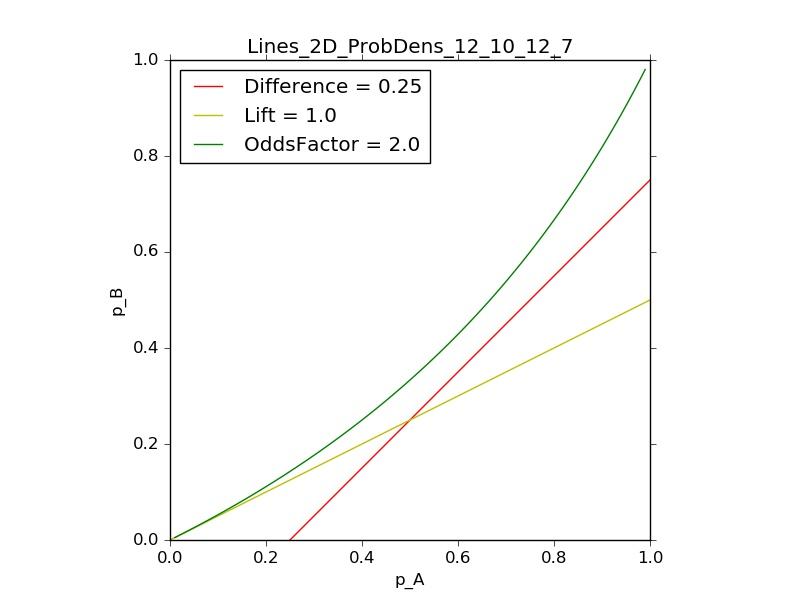
\includegraphics[width=90mm]{figures/metric_lines}
\caption{Probability Comparison Metrics on 2D Probability
  space \label{fig:metric_lines}}
\end{figure}
We recommend A over B if the
observed probabilities lie below and to the right of the chosen line.

Which metric captures the business interest?  Consider a Binary A/B
test in which the probability being measured is the {\em page
  transition probability} \(\tau\), that of moving to any other page
on the website as opposed to leaving the website or otherwise ending
the session. The business impact is {\em not} proportional to an
increase in the page transition probability. In most situations we
know that on average revenue is linear in clicks, conversions or other
monetizing actions, and that the number of these actions is linear in
the number of opportunties to act, which in turn is proportional
to the pages visited on the website. How is the number of page visits
\(P\) related to the page transition probability \(\tau\)? Some
thought shows that the average number of pages visited per
user-session is
\bdm
P= \tau + \tau^2 + \tau^3 + ...=
\frac{\tau}{1-\tau}
\edm
which is simply the {\em odds ratio} corresponding to the probability!

The preceding considerations show that we need an A/B analysis
framework that allows for new metrics. In this blog we will illustrate
our approach using the above odds ratio or page views metric. Further,
we will show how to get to a definite recommendation based on data and
a pre-established {\em Acceptance} factor \(\phi_{Acc}\) corresponding
to a doubling of the page views, without any ``confidence levels''
clouding the issue.

We are all aware of the inadequacies of the Frequentist approach with
its usual underlying assumption of normality (and concommitant
difficulties in dealing with ``small data''). Even if the
probabilities are normally distributed, the page visits are not since
they are non-linear in the probabilities. Within the Frequentist
framework, this would necessitate yet another difficult approximation.

For these reasons, we've taken a Bayesian approach: we use the data
from the experiment to construct the posterior probability
distribution (or likelihood) on 2 dimensional probability space. See
Fig.~\ref{fig:Bayes_line}, which shows a contour plot of the likelihood
for \((n_A, m_A, n_B, m_B) = (12,10,12,7)\), with the line
corresponding to a doubling of page views superimposed.
\begin{figure}[ht!]
\centering
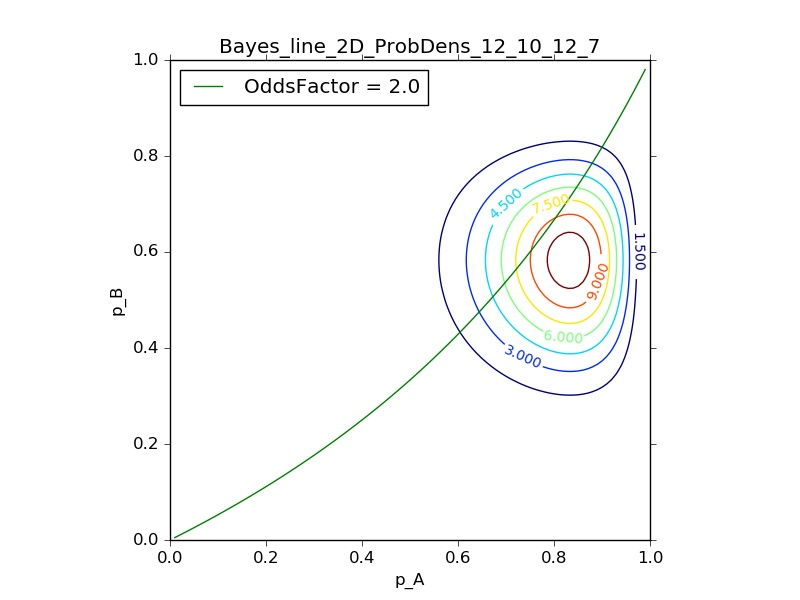
\includegraphics[width=90mm]{figures/Bayes_line}
\caption{Credibility = Volume of Prob. Density Below the Metric Line
  \label{fig:Bayes_line}}
\end{figure}
The contours correspond to points of equal probability density, with
the peak at \((10/12, 7/12)\).

Note that to compare with the metric line, we do not have a point
\((p_A,p_B)\) that corresponds to our knowledge of the success
probabilities, instead we have the 2 dimensional likelihood. Thus, we
can ask for the {\em probability} that \((p_A,p_B)\) lies below (and
to the right of) the metric line for a specific value of the metric,
Figure~\ref{fig:Bayes_line}.  This is simply the volume of the
likelihood function below the metric line for \(\phi\), and is
called the {\em credibility} of the result.

We analytically reduce the double integral involved to 1 dimension,
and then do a cute trick that allows for an easy numerical integration. So for
any value of the metric \(\phi\) we obtain its credibility.  For
concreteness, consider experimental results \((n_A, m_A) = (200, 40)\)
and \((n_B, m_B) = (100, 15)\). The analysis we've described so far
provides a {\em Page Views Lift vs. Credibility} curve based on the
experimental data, of the form in Figure~\ref{fig:odds_vs_cred}.
\begin{figure}[ht!]
\centering
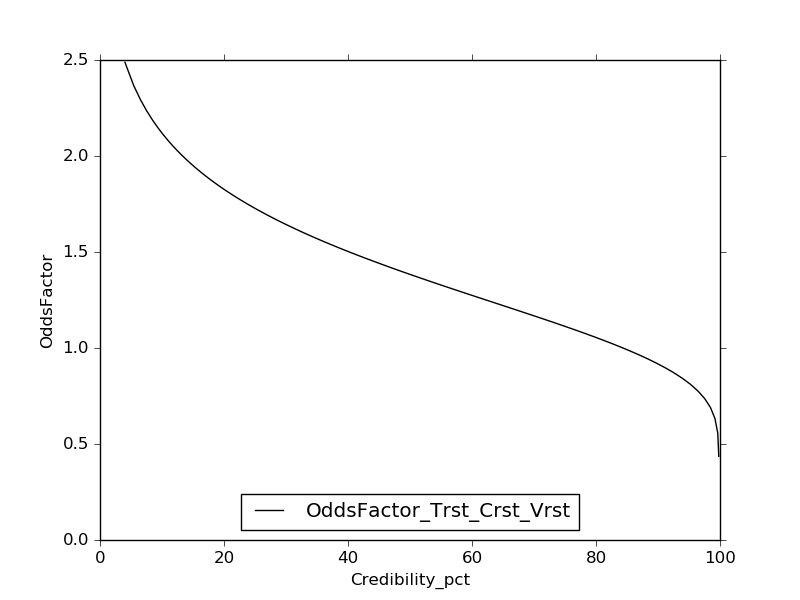
\includegraphics[width=90mm]{figures/OddsFactor_Trst_Crst_Vrst}
\caption{Page Views Lift vs. credibility \label{fig:odds_vs_cred}}
\end{figure}
which as expected is sigmoidal. Thus, we use the data to infer not
just {\em which treatment is better}, but in addition {\em by how
  much} and {\em how certain we are of this}.

This still does not help either us or the HiPPO, who needs a page
views lift of \(100\%\) (corresponding to \(\phi_{Acc}=2\)) to make a
decision. The constant expectation curve for \(\phi\)
\bdm
\phi* Cred(\phi) = \phi_{Acc}
\edm
is a hyperbola which can simultaneously lie in both the decision
halves of the plane that the metric vs. credibility curve
defines. This leads to contradictory recommendations for the same
business impact depending on the specific point chosen to represent
the business need.

Our approach to resolving this conundrum is to interpret
\(\phi*Credibility \) as the {\em expected minimum value} of
\(\phi\). We plot this as a function of the credibility in
Figure~\ref{fig:exp_odds_vs_cred}.
\begin{figure}[ht!]
\centering
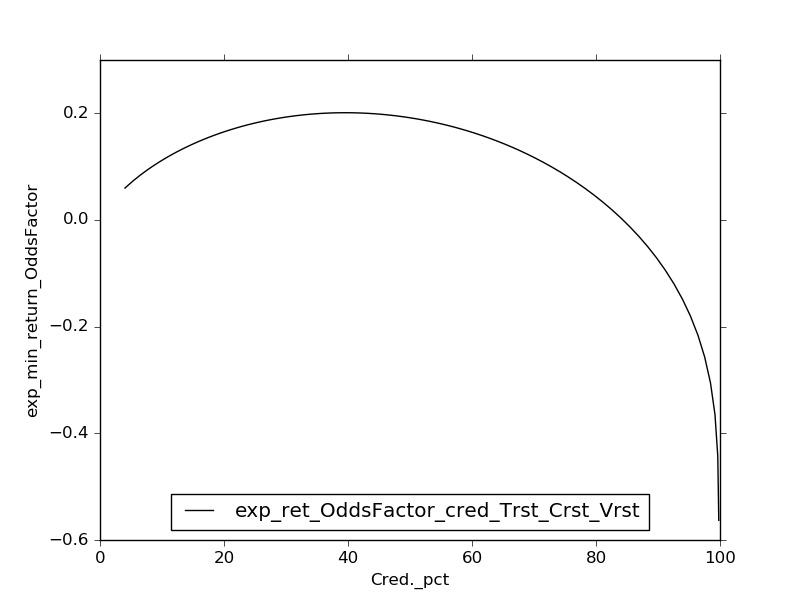
\includegraphics[width=90mm]{figures/exp_ret_OddsFactor_cred_Trst_Crst_Vrst}
\caption{Expected Minimum Odds Lift vs. Credibility \label{fig:exp_odds_vs_cred}}
\end{figure}
This expected minimum value has a maximum. The question of what recommendation to make is then
reduced to comparing the experimentally determined {\em maximum
  expected minimum value} to the client's acceptable value: if the
{\em max-min} is lower than the \(\phi_{Acc}\) then the variant is
{\em not} better than the control. Conversely,
\bdm
    {\rm If}\quad Max(Expected\quad Minimum\quad\phi) > \phi_{Acc},\quad {\rm then\quad we\quad recommend\quad A\quad over\quad B.}
\edm

\end{document}

